\chapter{Stacklook}
\label{lookin-at-stacks}
Tato kapitola se zabývá pluginem pro KernelShark, díky kterému bude jednodušší analyzovat trasovací data, kde se zachytával zásobník kernelu. V kapitole se seznámíme s cíli, analýzou řešení, návrhem a použitím tohoto pluginu. Nakonec i řešení kriticky zhodnotíme a představíme návrhy pro rozšíření.

\section{Cíle}

\begin{itemize}
    \item Nad podporovanými záznamy bude klikatelný objekt - po dvojitém kliknutí se zobrazí vyskakovací okénko.
    \item Tlačítka se budou zobrazovat nad záznamy jak v CPU grafech, tak v grafech procesů.
    \item Ve vyskakovacím okénku se zobrazí záznam zásobníku, název procesu, kterému událost záznamu patří a nějaká bližší informace specifická pro událost, nad kterou bylo tlačítko zobrazeno.
    \item Plugin bude mít konfigurační okénko, kde bude možné některé části chování upravit. Minimální součástí musí být zapínání a vypínání kreslení tlačítek nad podporovanými záznamy, úprava barev tlačítek a nastavování maximálního počtu viditelných záznamů v grafu, při jehož překročení se tlačítka nebudou zobrazovat.
    \item Informační řádek bude schopen zobrazit část zásobníku při přejetí kurzoru myši přes tlačítko. Která část zásobníku se zobrazí bude nastavitelné v konfiguraci pluginu. Jelikož informační řádek nemůže být změněn přes rozhraní pluginů a grafové objekty pluginů nereagují na přejetí myší, toto budou dodatečné modifikace, resp. modifikace \emph{Preview Labels Changeable} a \emph{Mouse Hover Plot Objects}.
    \item Tlačítka mohou být barevná stejně jako je zabarven proces, kterému záznam pod tlačítkem náleží. Získání barev procesů, CPU a streamů není v KernelSharku možné, KernelShark dovoluje barevné tabulky jenom vytvořit nanovo, které ovšem nebudou synchronizovány s tabulkami využívanými KernelSharkem. Zpřístupnění těchto tabulek bude dodatečná modifikace s názvem \emph{Get Colors}.
    \item Je nutné podporovat alespoň události typu sched/sched\_switch a sched/sched\_waking.
    \item Plugin bude možné používat i pro KernelShark bez modifikací vytvořených jako součást této práce.
\end{itemize}

Poslední bod existuje pro případné uživatele, kteří nechtějí používat modifikovaný KernelShark, dokud nejsou modifikace součástí oficiálního vydání. Plugin se tak může využívat i v úplné izolaci od ostatních změn z této práce, což souhlasí s obecnými požadavky na pluginy. Ostatní cíle vychází z kapitoly \emph{Obecná analýza a stanovení požadavků}. Jako samozřejmost se bere technická a uživatelská dokumentace a splnění obecných požadavků na pluginy.

\section{Analýza}
Tato sekce se pokusí zachytit postup, kterým se dostaneme k implementaci řešení. Jedná se o techničtější analýzu než analýza z kapitoly \emph{Obecná analýza a stanovení požadavků}.

\subsection{Propojení pluginu s KernelSharkem}
Zamysleme se nyní nad tím, jak bychom vytvořili plugin pro KernelShark s našimi cíli. Nejlepším začátkem by bylo nechat se inspirovat oficiálními pluginy, od nich se lze naučit, jak plugin propojit s KernelSharkem. Oficiální pluginy definují hlavičkový soubor v jazyce C, kde se definuje kontext pluginu. Tento kontext je pak struktura s globálně přístupnými daty pro plugin. S kontextem se i deklarují kontextové funkce ovládající jeho inicializaci a destrukci přes KernelSharkem definované makro. Krom toho se zde deklarují i další globálně přístupné prvky, které nevyžadují funkcionality C++. Tento hlavičkový soubor může své části implementovat jak C kódu, tak v C++ kódu. Oficiální pluginy mají v C napsanou hlavně definici kontextových funkcí, registraci handlerů pro různé události během načítání trasovacích dat, registrace handlerů na kreslení do grafu, inicializaci dat pro textový font a inicializaci ukazatelů na hlavní okno. Handlery jsou buď implementovány v C++, nebo, hlavně u jednoduchých handlerů událostí, ještě v implementačním C souboru. Kód napsaný v C je tedy většinou použit na inicializaci pluginu a další části, většinou s komplikovanější business logikou, jsou implementovány v C++.

Postup oficiálních pluginů je dobrý, využijeme jej tedy též. Stacklook ovšem bude vyžadovat více C++ kódu. Jednotlivé soubory pak budou sloužit jednotlivým modulům Stacklooku, například modul konfigurace bude obsahovat datovou struktury či datové struktury, které konfiguraci tvoří. Pokud možno, hlavičkové soubory by pak měly reprezentovat každý jeden z modulů. Podobné postupy jsou hojně využívány, hlavně při dekompozicích souboru s kódem, který obsahuje vícero modulů najednou.

\subsection{Analýza modulů řešení}
Z našich cílů lze celkem přímo vymezit moduly, ze kterých se bude plugin skládat: \emph{Propojující modul}, \emph{Konfigurace}, \emph{Tlačítka}, \emph{Detailní pohledy}.

\subsubsection{Propojující modul}
Propojující modul máme zčásti navržen díky oficiálním pluginům. V \uv{C části} (napsaná v jazyce C) nastavíme textový font používaný v pluginu, vybereme podporované události při načítání dat a registrujeme handlery. V \uv{C části} zároveň inicializujeme pluginový kontext. Tato část bude mít za úkol tento kontext i správně odstranit. V \uv{C++ části} definujeme handlery pro kreslení a přístup k hlavnímu oknu. Kreslící handler bude vyžadovat funkci na vytvoření tlačítek, tedy zde se propojí tlačítkový modul. Funkce vytvoření tlačítek bude potřebovat data pro barvu tlačítek, ta je v konfiguraci, takže se zde objeví i konfigurační modul. Tento modul bude také obsahovat podporované události a bude je sbírat do dat v kontextu pluginu.

\subsubsection{Konfigurace}
Konfigurace bude rozdělená mezi GUI okno a datovou strukturu s konfiguračními daty, tzv. konfigurační objekt. Konfigurační objekt samotný implementujeme jako singleton. Důvodem je nutnost znát konfiguraci v různých částech programu a že konfigurace musí být vždy pouze jedna, což právě singleton splňuje. Prvky z cíle o konfiguraci můžeme jednoduše uložit jako čísla, pravdivostní hodnoty, textové řetězce a datovou strukturu pro barvy od KernelSharku. Aby bylo možné konfiguraci měnit pouze skrze konfigurační okno, tyto prvky schováme pomocí modifikátorů viditelnosti. Konfigurační objekt pak využije C++ mechanismus \uv{spřátelení} přes klíčové slovo \texttt{friend} a označí konfigurační okno za svého přítele. Konfigurace pluginů KernelSharku nejsou persistentní, tak dodáme i nějaké výchozí hodnoty. Kvůli zobrazování zásobníku v informačním řádku, přidáme ke každému nastavení specifickému pro událost i offset od vrchu zásobníku. Tak budeme moci stanovit oblast zásobníku, ve které se většinou nachází ty nejzajímavější části zásobníku pro danou událost.

Konfigurační okno využije framework Qt (specificky Qt6), stejně jako ostatní grafické prvky KernelSharku. Na barevná nastavení vytvoříme tlačítko, které na kliknutí vyvolá nějaké okno na výběr barvy, například výchozí barevný dialog od Qt. Pro pohodlí uživatele i někde blízko tlačítka výběru barvy zobrazíme i aktuálně použitou barvu. Nastavení maximálního počtu viditelných záznamů lze reprezentovat jako spinbox. Konfigurace pro specifické události, tj. zdali nad danými událostmi zobrazovat tlačítka nebo offset použitý při zobrazování části zásobníku v informačním řádku, lze reprezentovat pomocí zaškrtávacího tlačítka a dalšího spinboxu. Mimo požadavky navíc dodáme zaškrtávací tlačítko pro barvení tlačítek barvami jejich procesů.

\subsubsection{Tlačítka}
Modul tlačítek se bude hlavně skládat z třídy pro tlačítka. Ta by měla být v grafu jasně viditelná a ihned rozpoznatelná uživatelem. Tvar tlačítek by měl nějak ukazovat, kterému záznamu patří. Zde je několik možností a tvarů na výběr, nicméně nejjednodušším tvarem bude trojúhelník. Jeden z vrcholů bude směřovat dolů, ostatní dva vrcholy budou nad tímto vrcholem. Rozpoznatelnost těchto tlačítek nakonec zajistíme přidáním nápisu \texttt{STACK} do každého z nich. Reakci na dvojité kliknutí a přejetí kurzorem myši implementujeme jako to dělají ostatní tvary definované KernelSharkem. U přejetí využijeme naše modifikaci na reakci na přejetí kurzorem myši a modifikaci na změnu informačního řádku, přesně jak říká jeden z cílů. Speciálně pro sched\_switch budou tlačítka ještě obsahovat jedno písmeno symbolizující předchozí stav procesu před přepnutím. Takto nebude nutné se podívat do detailního pohledu, bude stačit se dívat do grafu. Nicméně uživatel bude muset znát zkratky pro možné předchozí stavy. Ty jsou součástí dokumentace Linuxu \cite{Process-State-Codes}, společně s méně známým stavem \uv{parked} \cite{Parked-Thread}. Barva tlačítek bude určena hodnotami v konfiguračním objektu. Dodáme i možnost používat barvy procesů jako barvy tlačítek, to nám zajistí modifikace \emph{Get Colors}. Aby nemohlo více tlačítek splývat díky stejné barvě, tlačítka budou mít obrys, jehož barva bude také dána konfigurací a bude oddělená od (vnitřní) barvy tlačítka.

\subsubsection{Detailní pohledy}
Modul detailních pohledů bude hlavně obsahovat třídu pro okna těchto pohledů. V okně pak zobrazíme záznam zásobníku ve formě seznamu. Tento formát se hodí na jednoduché zvýraznění položky jedním kliknutím. Dodáme ale i možnost si data zobrazit jako prostý text - tento formát je naopak lepší když se kopírují data po jných částech než po položkách. Na vrchol zásobníku dodáme značku \texttt{top}, aby bylo jasné, kde se vrch zásobníku nachází. Jeden z cílů nám ještě udává nutnost zobrazit název procesu a nějaké bližší informace o události. Pro sched\_switch zde můžeme udat předchozí stav procesu před přepnutím, například zdali byl proces již ve stavu zombie, nebo zdali začal čekat na nějaká data a nebo zdali prostě běžel a byl preemptivně přepnut. Předchozí stav zapíšeme jak zkratkou, tak celým názvem (například \uv{S - sleep}, nebo \uv{Z - zombie}). Pro sched\_waking pouze napíšeme, že byl proces probuzen. Nakonec se zamyslíme nad tím, jak dlouho budou okna žít a kolik jich může být najednou pro jednu událost. Naše pohledová okna můžeme vytvořit jako podřízená oknu hlavnímu, tedy pokud je ukončeno hlavní okno, budou ukončena i jeho podřízená okna. Toto zajistí Qt framework. Počet oken pro jednu událost nebudeme omezovat, nic se tím nerozbije a implementace bude jednodušší. Tato rozhodnutí by měla mít ten efekt, že uživatel bude schopen stream, nazvěme jej A, pak bude schopen začít zkoumat stream jiný, nazvěme tento B. Okna otevřená ve streamu A zůstanou otevřená i po přepnutí do streamu B, do té doby dokud je uživatel sám nezavře, nebo dokud uživatel nezavře hlavní okno. Lze tak porovnávat zásobníky z různých běhů trasování.

\subsubsection{Předchozí stavy}
Na získání informací o předchozím stavu ještě dodáme mini-modul \emph{Předchozí stavy}. Nutně bude muset být schopen vytáhnout data o předchozím stavu ze záznamu události přepnutí v KernelSharku. Tato data pak bud muset umět dodat pluginu buď jako zkratka pro typ stavu (tlačítka a detailní pohledy), nebo jako celý název (detailní pohledy).

\subsection{Údaje v informačním řádku}
Postupujme dále, podívejme se na informační řádek. Informační řádek nabízí pouze pět míst pro text. Pokud bychom museli zobrazovat konec zásobníku, nebo i prvky za koncem (například kvůli vysokému offsetu v konfiguraci), v informačním řádku pak vyznačíme, že jsme na konci zásobníku a místa, kde by byly prvky za koncem označíme nějakou čárou, třeba mínusem. Pokud ale zobrazujeme oblast zásobníku a za ní zásobník pokračuje, označíme toto třemi tečkami v posledním místě pro text v informačním řádku. Nakonec, pro jasnou identifikaci procesu z jehož záznamu zásobníku čerpáme bude první místo v informačním řádku obsazeno názvem tohoto procesu. Prvky v informačním řádku tedy budou vždy v následujícím pořadí:
\begin{itemize}
  \item Název procesu
  \item Věc na zásobníku na offsetu X od vrcholu zásobníku, nebo \texttt{-}
  \item Věc na offsetu X+1, nebo \texttt{-}
  \item Věc na offsetu X+2, nebo \texttt{-}
  \item \texttt{...}, nebo \texttt{(End of stack)}
\end{itemize}
Informační řádek bude vždy schopen zobrazit nejvýše tři prvky ze zásobníku.

\subsection{Získání záznamů zásobníku}
Nakonec se zamyslíme, jak získat data záznamů zásobníku kernelu. Tlačítka jsou nad záznamy, po kterých následuje záznam zásobníku. Tyto záznamy se vždy vytvoří na stejném CPU jako událost jim předcházející. Během načítání dat ale ještě nemáme události seřazené, ovšem při prvním kreslení už ano. Navíc neplatí, že všechny soubory trasovacích dat musí obsahovat záznamy zásobníku, lze systém trasovat i bez sbírání zásobníku. V tom přípaě nemá smysl, aby plugin cokoli kreslil. Do kontextu pluginu dodáme dvě proměnné, jednu jako indikátor \uv{hledali jsme záznam trasování zásobníku kernelu} a druhou jako \uv{záznam trasování zásobníku existuje}, přičemž obě začnou na pravdivostní hodnotě \uv{nepravda}. Při prvním kreslení prohledáme následníky všech záznamů námi podporovaných událostí. Pokud alespoň jeden záznam má za následníka záznam zásobníku, nastavíme druhou proměnnou v kontextu na \uv{pravda}. Ukazatel na tento záznam si pak poznamenáme i u záznamu předcházející události. Po prohledání všech podporovaných záznamů nastavíme i první proměnnou na \uv{pravdu}. Tak si zajistíme jediný chod při hledání těchto dat. Ačkoliv prohledávání může trvat dlouho, stane se tak pouze jednou a časová cena prohledávání tak není příliš výrazná.

\subsection{Plugin pro nemodifikovaný KernelShark}

Každá část implementace využívající nějakou z našich modifikací bude obalena podmínkovým \texttt{ifndef} makrem s názvem \texttt{\_UNMODIFIED\_KSHARK}. Toto makro bude aktivováno pokud uživatel při sestavování tuto proměnnou definuje argumentem pro CMake, více v uživatelské dokumentaci v sekci o instalaci. Pokud je makro definováno, pak zvolí alternativní implementaci z \texttt{else} větve, která nevyužívá žádnou z modifikací; jinak kód nebude součástí kompilace.

\section{Vývojová dokumentace}

\subsection*{Dokumentace pluginu}
Dokumentace je napsána pro nástroj Doxygen. Dokumentovala se každá funkce i proměnná, nicméně vygenerovaná dokumentace obsahuje jenom prvky veřejné, pro skutečné implementační detaily je tedy doporučeno se podívat do zdrojového kódu. Dokumentace navíc obsahuje hlavní stránku a stránku s nástinem návrhu.

\subsection*{Struktura projektového adresáře}

Adresář pluginu obsahuje další adresáře. Adresář \uv{src} je pro zdrojový kód a adresář \uv{doc} je pro dokumentaci uživatelskou a dokumentaci technickou. Očekává se, že na této úrovni jsou i adresáře pro sestavení. Na stejné úrovni žije i README, soubor s licencí a nejvyšší CMakeLists.txt. V těchto CMake instrukcích se nastaví proměnné sestavení, například typ sestavení, a případně se zavolá generování dokumentace. CMake instrukce zodpovědné za vytvoření binárního souboru jsou v adresáři se zdrojovým kódem, stejně jako to dělá KernelShark.

\subsection*{Struktura pluginu}
Plugin rozdělíme na moduly. Pro detailnější informace a implementační detaily je doporučeno prohlédnout si samotný kód a technickou Doxygen dokumentaci pluginu.

Ke každému modulu připíšeme i soubory, ve kterých je modul implementován, a prvky modulu jako veřejné funkce, makra, či veřejné datové struktury. Prvky mimo hlavičkové soubory, nebo označeny za privátní pro třídu jsou brány jako implementační detaily a nebudou zde popsány (lze je najít uvnitř souborů modulu).

\subsubsection*{Propojující modul}
Modul s kódem propojujícím KernelShark a plugin. Obsahem je hlavně kontext pluginu, funkce kontextu, handlery a implementačně pomocné funkce. Součástí tohoto modulu je část s C kódem a implementační část v C++ prvků z hlavičkového C souboru. Právě v \uv{C++ části} (napsaná v C++) se ostatní moduly propojují; zároveň tato část ukládá některá globální data s C++ typy.

\begin{itemize}
  \item \textbf{Soubory:} stacklook.h/c, Stacklook.cpp
  \item \textbf{Datová struktura:} kontextová struktura \emph{plugin\_stacklook\_ctx} s identifikátory, řídícími proměnnými a kolekcí zajímavých záznamů událostí.
  \item \textbf{Makra:}
  \begin{itemize}
    \item \emph{FONT\_SIZE} - udává velikost textů vytvořených pluginem.
    \item \emph{KS\_DECLARE\_PLUGIN\_CONTEXT\_METHODS} - deklaruje generické funkce pro inicializaci, uzavření a pro získání kontextu pluginu.
  \end{itemize}
  \item \textbf{Funkce:}
  \begin{itemize}
    \item \emph{get\_font\_ptr} - získá ukazatel na textový font.
    \item \emph{get\_bold\_font\_ptr} - získá ukazatel na tučný textový font.
    \item \emph{get\_kstack\_entry} - získá nejbližší záznam události záznamu zásobníku kernelu.
    \item \emph{draw\_stacklook\_objects} - handler pro kreslení Stacklook tlačítek.
    \item \emph{plugin\_set\_gui\_ptr} - předá Stacklooku ukazatel na hlavní okno KernelSharku během inicializace pluginu.
  \end{itemize}
  \item Další části modulu jsou brány jako implementační detaily.
\end{itemize}

\subsubsection*{Konfigurace}
Modul řeší současná nastavení Stacklooku, jejich vizuální stránku, přístupy ke konfiguračním hodnotám a jejich změny.

\begin{itemize}
  \item \textbf{Soubory:} SlConfig.hpp/cpp
  \item \textbf{Třídy:}
    \begin{itemize}
      \item \emph{SlConfig} - singleton, obsahuje konfigurační data, která plugin zrovna využívá.
      \item \emph{SlConfigWindow} - GUI element, přes který lze měnit data v konfiguračním objektu.
    \end{itemize}
  \item \textbf{Typové aliasy:}
    \begin{itemize}
      \item \emph{allowed\_t} - pro označení povolení zobrazovat nad záznamem události tlačítko. Pro nemodifikovaný Stacklook je toto zároveň jediná konfigurace Stacklooku specifická pro každou podporovanou událost.
      \item \emph{event\_name\_t} - pro označení názvu události.
      \item \emph{events\_meta\_t} - pro označení vazby událostí a konfigurací Stacklooku pro ně specifických.
    \end{itemize}

    Pro modifikovaný KernelShark ještě:
    \begin{itemize}
      \item \emph{depth\_t} - pro označení počáteční hloubky/offsetu do zásobníku.
      \item \emph{event\_meta\_t} - pro označení konfigurace Stacklooku specifické pro nějaký plugin, která obsahuje vedle povolení zobrazovat nad záznamem události tlačítko udržuje i offset do zásobníku.
    \end{itemize}
  \item Další části modulu jsou brány jako implementační detaily.
\end{itemize}

\subsubsection*{Tlačítka}
Modul řeší interaktivní tlačítka, která jsou vykreslována v grafu nad záznamy podporovaných událostí a jejich interakce.

\begin{itemize}
  \item \textbf{Soubory:} SlButton.hpp/cpp
  \item \textbf{Třída:} grafický prvek \emph{SlTriangleButton}, vykreslován do grafu trasování, dokáže reagovat na přejetí kurzorem myši a dvojité klikntí.
  \item Další části modulu jsou brány jako implementační detaily.
\end{itemize}

\subsubsection*{Detailní pohledy}
Modul řeší detailní pohledy, tj. grafická okna pro podrobnější pohled na záznam zásobníku kernelu.

\begin{itemize}
  \item \textbf{Soubory:} SlDetailedView.hpp/cpp
  \item \textbf{Třída:} grafické okno \emph{SlDetailedView} zobrazující zaznamenaný kernel zásobník, informace o události, která záznamu zásobníku předcházela, a informace o procesu vlastnící tuto událost.
  \item Další části modulu jsou brány jako implementační detaily.
\end{itemize}

\subsubsection*{Předchozí stavy}
Mini-modul, dodává data tlačítkům a detailním pohledům o stavu procesu před přepnutím kontextu na CPU.

\begin{itemize}
  \item \textbf{Soubory:} SlPrevState.hpp/cpp
  \item \textbf{Statická konstanta:} nová konstanta \emph{LETTER\_TO\_NAME} je mapou zkratek jmen předchozích stavů na jejich celá jména.
  \item \textbf{Funkce:} 
  \begin{itemize}
    \item \emph{get\_switch\_prev\_state} - vrátí zkratku jména předchozího stavu ze záznamu pro sched\_switch událost.
    \item \emph{get\_longer\_prev\_state} - vrátí celé jméno předchozího stavu ze záznamu pro sched\_switch událost.
  \end{itemize}
\end{itemize}

\section{Uživatelská dokumentace}

Tato sekce popíše jak instalovat a používat plugin Stacklook v KernelSharku a co od něj během běhu očekávat, či na co si dát pozor. Obrázek \ref{SlWorking} ukazuje fungující plugin v akci. Styl a i obsah této dokumentace jsou velmi podobné uživatelské dokumentaci pluginu Naps, jelikož jsou efektivní a dají se jednoduše poupravit na jiný plugin.

\begin{figure}[p]\centering
    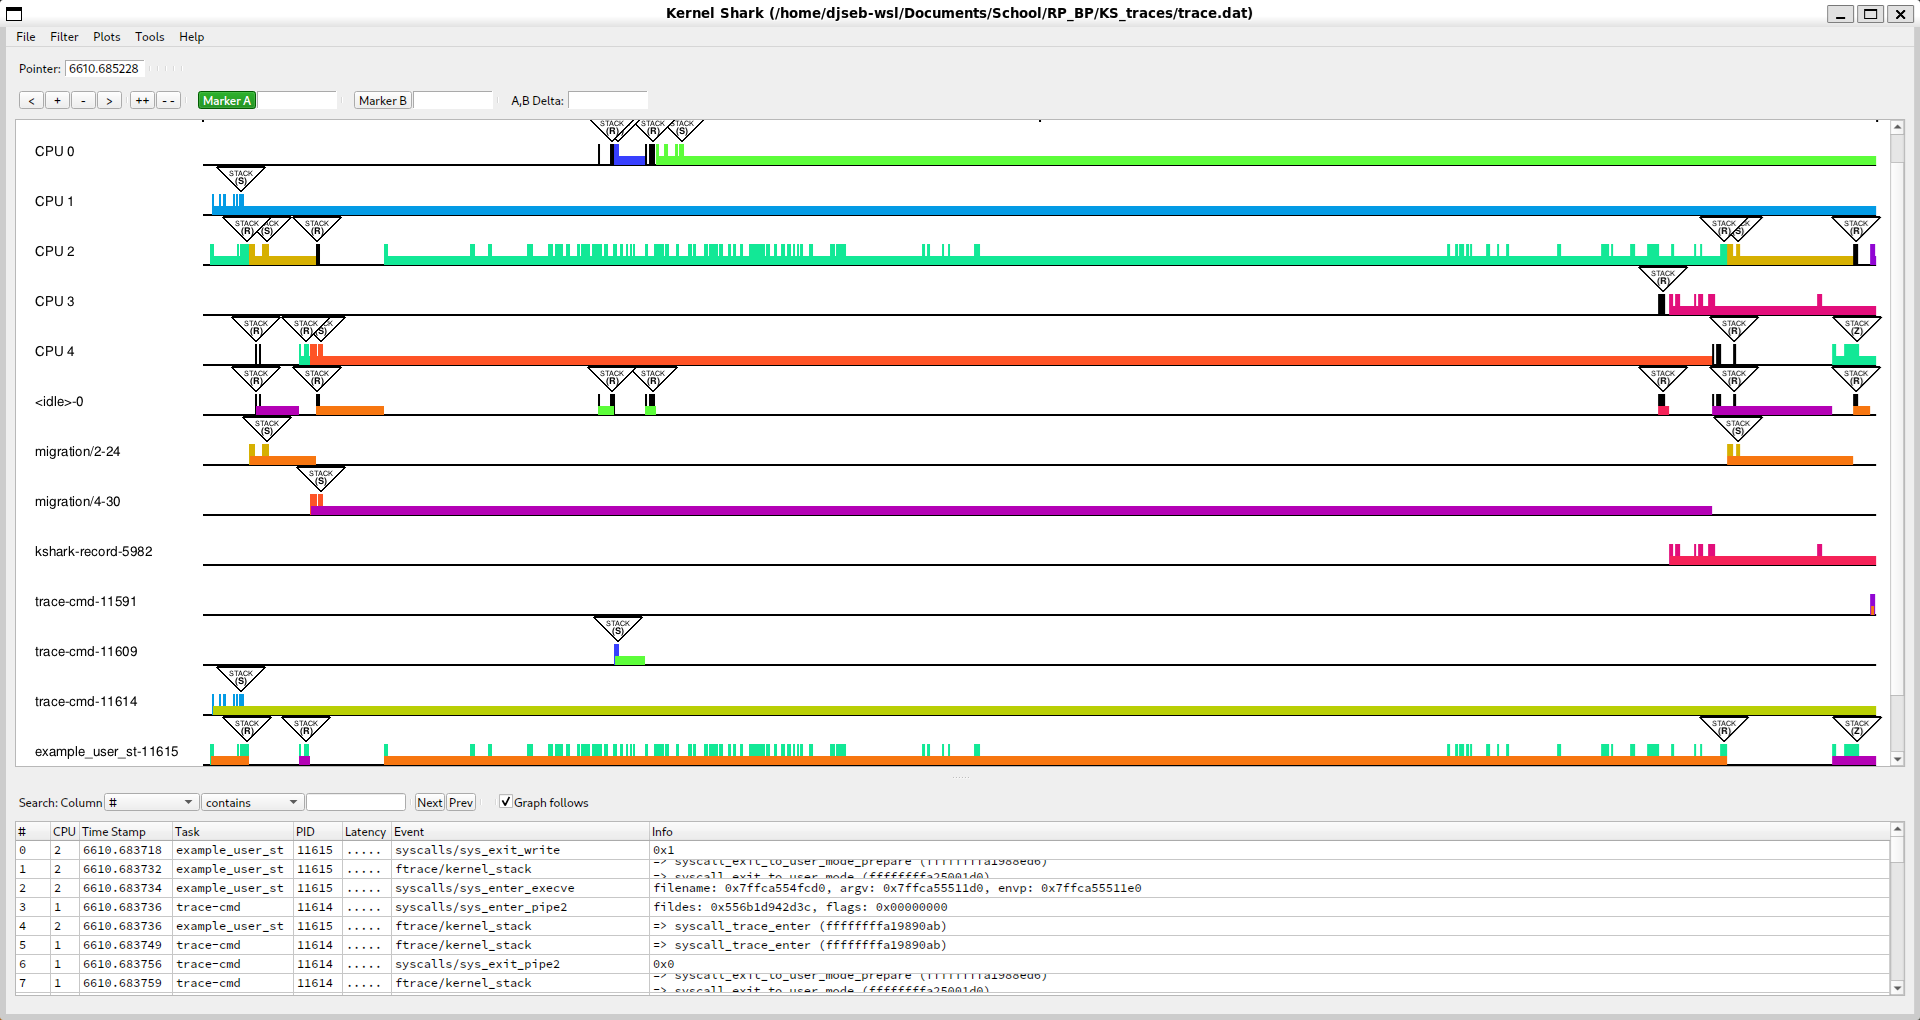
\includegraphics[width=140mm]{img/Stacklook/SlWorking}
    \caption{Fungující Stacklook}
    \label{SlWorking}
\end{figure}

\subsection{Jak sestavit a instalovat Stacklook}

\subsubsection*{Předpoklady}

\begin{itemize}
  \item CMake verze alespoň 3.1.2.
  \item Pokud chceme plugin využívající modifikovaný KernelShark, pak je nutná verze alespoň 2.4.0-couplebreak. Pokud chceme plugin pro nemodifikovaný KernelShark, pak je nutná verze alespoň 2.3.2.
  \item Závislosti KernelSharku (nalezneme v README repozitáře KernelSharku), zejména Qt6.
  \item Doxygen na technickou dokumentaci.
\end{itemize}

\subsubsection{Sestavení a instalace pouze pluginu}

\begin{enumerate}
  \item V terminálu nastavme pracovní adresář na složku \texttt{build} (pokud ještě neexistuje, pak ji nejlépe vytvořme v kořenovém adresáři projektu).
  \item Spusťme příkaz \texttt{cmake ..}. Pokud hlavní soubor \texttt{CMakeLists.txt} není v nadřazené složce, předejme programu CMake platnou cestu k němu.
    \begin{itemize}
      \item Používáte-li verzi KernelSharku bez modifikací, přidejme do příkazu argument \texttt{-D\_UNMODIFIED\_KSHARK}.
      Sestavení pro nemodifikovaný KernelShark odstraňuje tyto funkce:
      \begin{itemize}
        \item Tlačítka mohou být stejné barvy, jako procesy, jimž patří záznamy s tlačítky.
        \item Přejetí myši zobrazí část zásobníku v informačním řádku KernelSharku.
      \end{itemize}
      \item Pokud chceme generovat dokumentaci pomocí Doxygenu, přidejme do příkazu argument \texttt{-D\_DOXYGEN\_DOC=1}.
      \item Výchozí typ sestavení je \texttt{RelWithDebInfo}. Chcete-li ho změnit (např. na \texttt{Release}), použijme argument \texttt{-DCMAKE\_BUILD\_TYPE=Release}.
      \item Pokud se soubory Qt6 nenacházejí ve \texttt{/usr/include/qt6}, použijme argument \texttt{-D\_QT6\_INCLUDE\_DIR=[PATH]}, kde \texttt{[PATH]} nahradíme cestou k souborům Qt6.
        \begin{itemize}
          \item Pokyny pro sestavení předpokládají, že zadaný adresář má stejnou vnitřní strukturu jako výchozí možnost (tj. obsahuje složky QtCore, QtWidgets apod.).
        \end{itemize}
      \item Pokud se zdrojové soubory KernelSharku nenachází v \texttt{../KS\_fork/src}, použijme argument \texttt{-D\_KS\_INCLUDE\_DIR=[PATH]}, kde \texttt{[PATH]} nahradíme cestou ke zdrojovým souborům KernelSharku.
      \item Pokud se sdílené knihovny KernelSharku (\texttt{.so} soubory) nenachází ve \texttt{/usr/local/lib64}, použijme \texttt{-D\_KS\_SHARED\_LIBS\_DIR=[PATH]} argument, kde \texttt{[PATH]} nahradíme cestou k sdíleným knihovnám KernelSharku.
    \end{itemize}
  \item Ve složce \texttt{build} spusťme příkaz \texttt{make}.
    \begin{itemize}
      \item Pokud je třeba sestavit jen část pluginu, například pouze dokumentaci, můžeme vybrat konkrétní cíl.
      \item Pouhé spuštění \texttt{make} vytvoří: \emph{plugin} (cíl \texttt{stacklook}), \emph{symlink} na sdílený objekt pluginu (cíl \texttt{stacklook\_symlink}) a případně \emph{Doxygen dokumentaci} (cíl \texttt{docs}), pokud tak bylo specifikováno v předchozím kroku.
    \end{itemize}
  \item (\emph{Instalace}): Nahrajme plugin do KernelSharku, buď přes GUI, nebo při spouštění přes CLI s argumentem \texttt{-p} a cestou k symlinku nebo přímo k sdílenému objektu.
    \begin{itemize}
      \item \emph{DŮLEŽITÉ}: Vždy nainstalujte/nahrajme plugin před načtením relace, ve které byl aktivní! Jinak může dojít k neúplnému načtení konfiguračního rozhraní nebo k pádu celého programu.
    \end{itemize}
\end{enumerate}

K odstranění vytvořených binárních souborů použijme \texttt{make clean}.

\subsubsection{Sestavení a instalace pomocí KernelSharku}

\begin{enumerate}
  \item Ujistěme se, že všechny zdrojové soubory (\texttt{.c}, \texttt{.cpp}, \texttt{.h}) Stacklooku se nacházejí ve složce \texttt{src/plugins} v adresáři projektu KernelShark.
  \item Zkontrolujme, že soubor \texttt{CMakeLists.txt} v této podsložce obsahuje instrukce pro sestavení pluginu (inspirovat se můžeme podle jiných pluginů pro GUI). Pokud chceme sestavovat pro nemodifikovaný KernelShark, upravme tomu odpovídajícím způsobem build skript.
  \item Sestavme KernelShark (pluginy se sestavují automaticky). Lze sestavit i pouze plugin, pokud jsme již předtím vytvořili instrukce sestavení.
  \item (\emph{Instalace}): Spusťme KernelShark. Pluginy sestavené tímto způsobem se načítají automaticky. Pokud by se z nějakého důvodu nenačetly, najděme sdílený objekt stejně jako u ostatních oficiálních pluginů, opět buď přes GUI, nebo přes CLI.
\end{enumerate}

\subsubsection{VAROVÁNÍ - načítání více verzí pluginu}

Máte-li dvě nebo více sestavených verzí pluginu, \emph{NE}načítejme je současně do KernelSharku. Pokud to uděláme, \emph{DOJDE K PÁDU PROGRAMU}. Používejme vždy jen jednu z verzí, \emph{NIKDY OBOJE NAJEDNOU}.

\subsection{Jak zapnout/vypnout Stacklook}

Zapnutí pluginu je velmi jednoduché. Stačí spustit KernelShark a přejít na položku v panelu nástrojů \texttt{Tools > Manage Plotting plugins}. Pokud byl plugin načten přes příkazový řádek, zobrazí se v seznamu pluginů jako zaškrtnuté políčko se svým názvem. Pokud ne, lze plugin dohledat pomocí tlačítka \texttt{Tools > Add plugin} - stačí nalézt symlink, ale je možné vybrat i samotný soubor sdíleného objektu. Jak je vidět, plugin využívá standardní mechanismus načítání pluginů v KernelSharku. Obrázek~\ref{SlManagePlottingPlugins} ukazuje GUI pro zapínání a vypínání pluginů.

\begin{figure}[p]\centering
    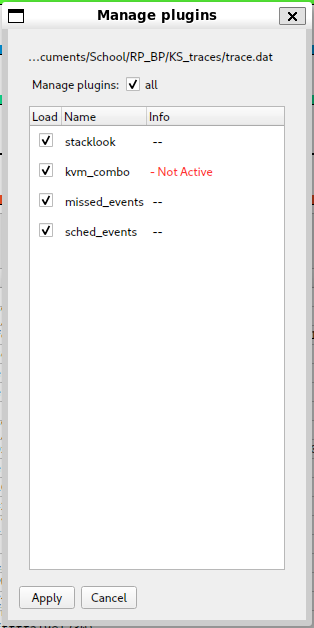
\includegraphics[height=140mm]{img/Stacklook/SlManagePlottingPlugins}
    \caption{Okénko se správou pluginů}
    \label{SlManagePlottingPlugins}
\end{figure}

\subsection{Jak používat Stacklook}

\subsubsection{Konfigurace}

Konfigurace pluginu může být provedena kdykoliv, i před načtením jakýchkoliv trasovacích dat. Pro otevření konfiguračního okna (viz obrázek~\ref{SlConfigWindow}) stačí v hlavním okně zvolit \texttt{Tools > Stacklook Configuration}. Vždy může být otevřeno jen jedno konfigurační okno.

\begin{figure}[p]\centering
    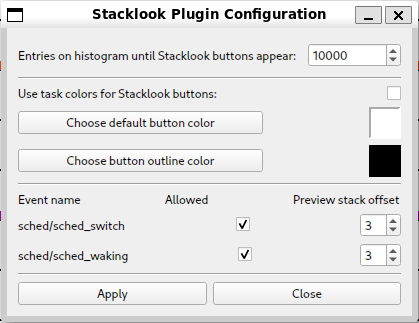
\includegraphics[width=140mm]{img/Stacklook/SlConfigWindow}
    \caption{Konfigurační okno Stacklooku pro modifikovaný KernelShark}
    \label{SlConfigWindow}
\end{figure}

Používáte-li verzi pluginu pro nemodifikovaný KernelShark, bude v konfiguračním okně chybět zaškrtávací políčko pro barvení tlačítek barvami procesů a nastavení offsetu, použitého při zobrazování prvků zásobníku v informačním řádku, viz obrázek~\ref{SlUnmodifiedKsharkConfigWindow}.

\begin{figure}[p]\centering
    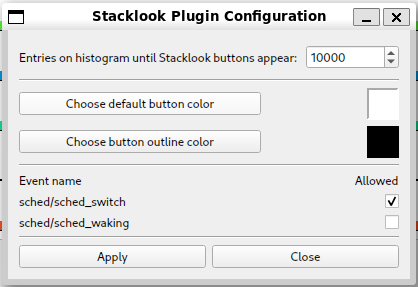
\includegraphics[width=140mm]{img/Stacklook/SlUnmodifiedKsharkConfigWindow}
    \caption{Konfigurační okno Stacklooku pro nemodifikovaný KernelShark}
    \label{SlUnmodifiedKsharkConfigWindow}
\end{figure}

Nyní si popíšeme jednotlivé možnosti konfigurace a jak je ovládat. Seřazeno shora dolů:
\begin{itemize}
  \item \emph{Limit záznamů v histogramu} - snížením této hodnoty omezíme, kdy se Stacklook aktivuje. Aktivace nastane pouze tehdy, pokud je viditelný počet záznamů menší nebo roven této hodnotě. Čím nižší číslo, tím větší přiblížení je třeba k aktivaci Stacklooku. Minimální hodnota je 0, maximální 1~000~000~000 (jedna miliarda), tato horní mez však bude pravděpodobně zřídka využita. Výchozí hodnota je 10~000 (deset tisíc).
  
  \item \emph{Použít barvy procesů pro tlačítka Stacklooku} - zaškrtnutím tohoto políčka (pokud je k dispozici) bude výplň tlačítek Stacklooku zabarvena barvou procesu, ke kterému patřila událost, pro niž Stacklook našel záznam zásobníku. Pokud políčko necháme nezaškrtnuté, použijí se barvy v konfiguraci Stacklooku (výchozí barvy na obrázku~\ref{SlDefaultColors}). Tato volba je ve výchozím stavu vypnutá.
  
  \begin{figure}[p]\centering
      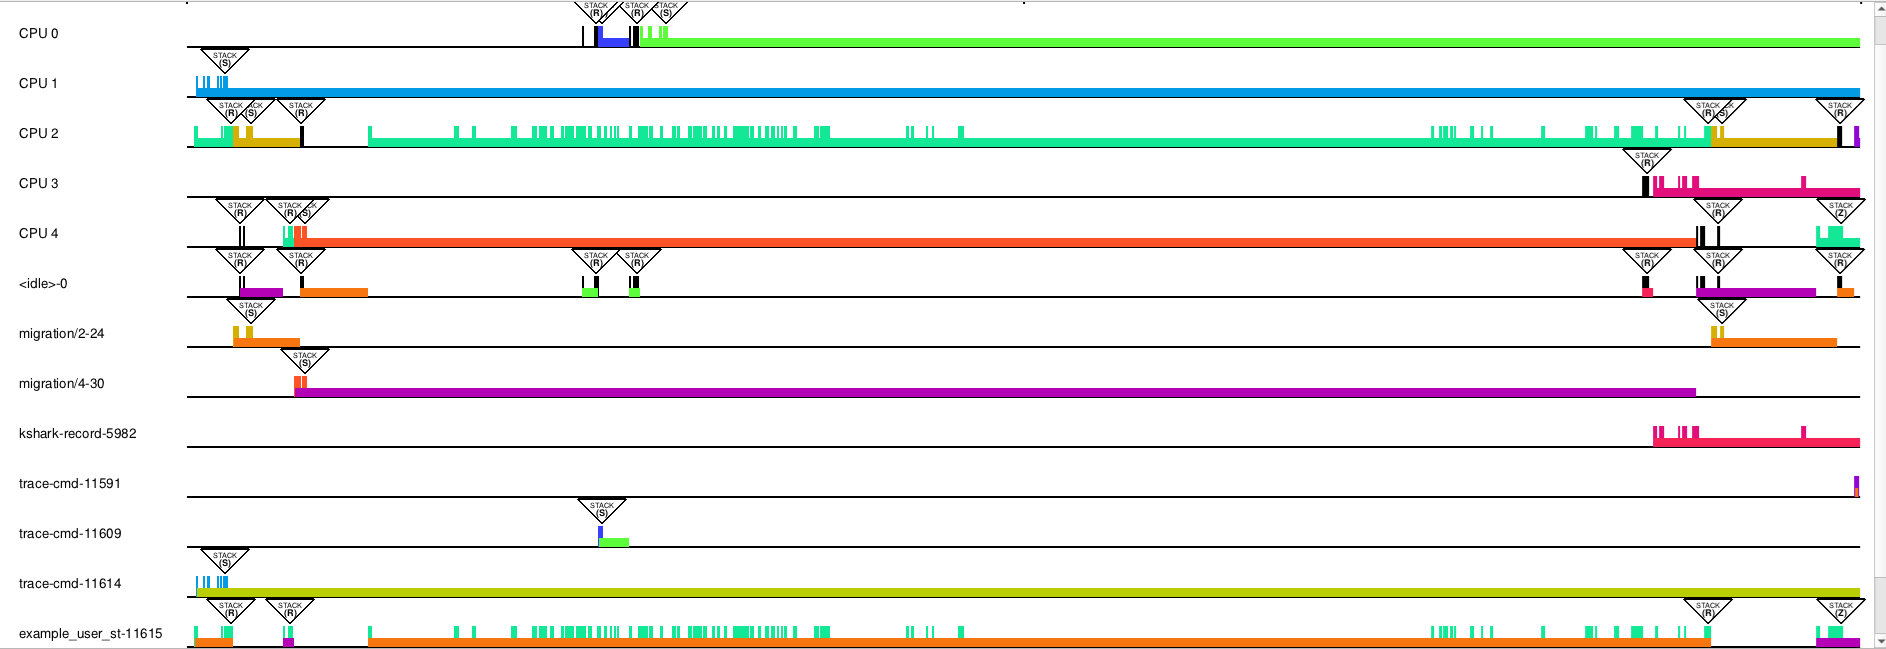
\includegraphics[width=140mm]{img/Stacklook/SlDefaultColors}
      \caption{Tlačítka s výchozími barvami}
      \label{SlDefaultColors}
  \end{figure}
  
  \begin{figure}[p]\centering
      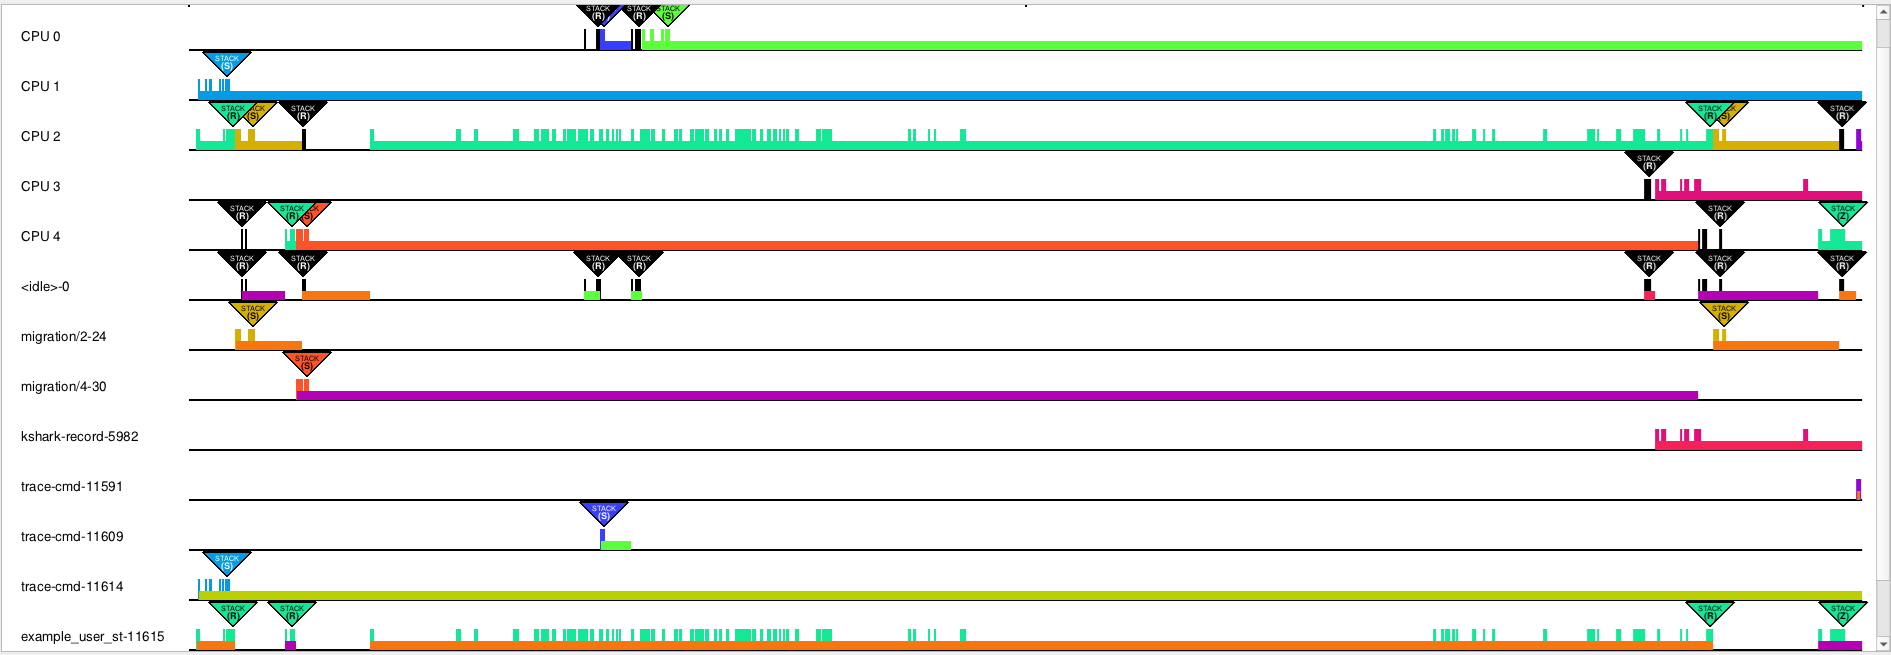
\includegraphics[width=140mm]{img/Stacklook/SlTaskColors}
      \caption{Tlačítka využívající barvy procesů}
      \label{SlTaskColors}
  \end{figure}

  \item \emph{Barvy tlačítek Stacklooku a jejich obrysů} - tlačítka \texttt{Choose} otevřou dialog pro výběr barev, kde lze nastavit barvu výplně tlačítka nebo jeho obrys. Tato nastavení mají účinek pouze tehdy, pokud není dostupná nebo není aktivní volba barev podle procesů. Vedle tlačítek je zobrazen náhled aktuálně vybraných barev. Výchozí nastavení je bílá výplň a černý obrys. Příklad jiných barev si lze prohlédnout na obrázku~\ref{SlCustomDefaultColors}.
  
  \begin{figure}[p]\centering
      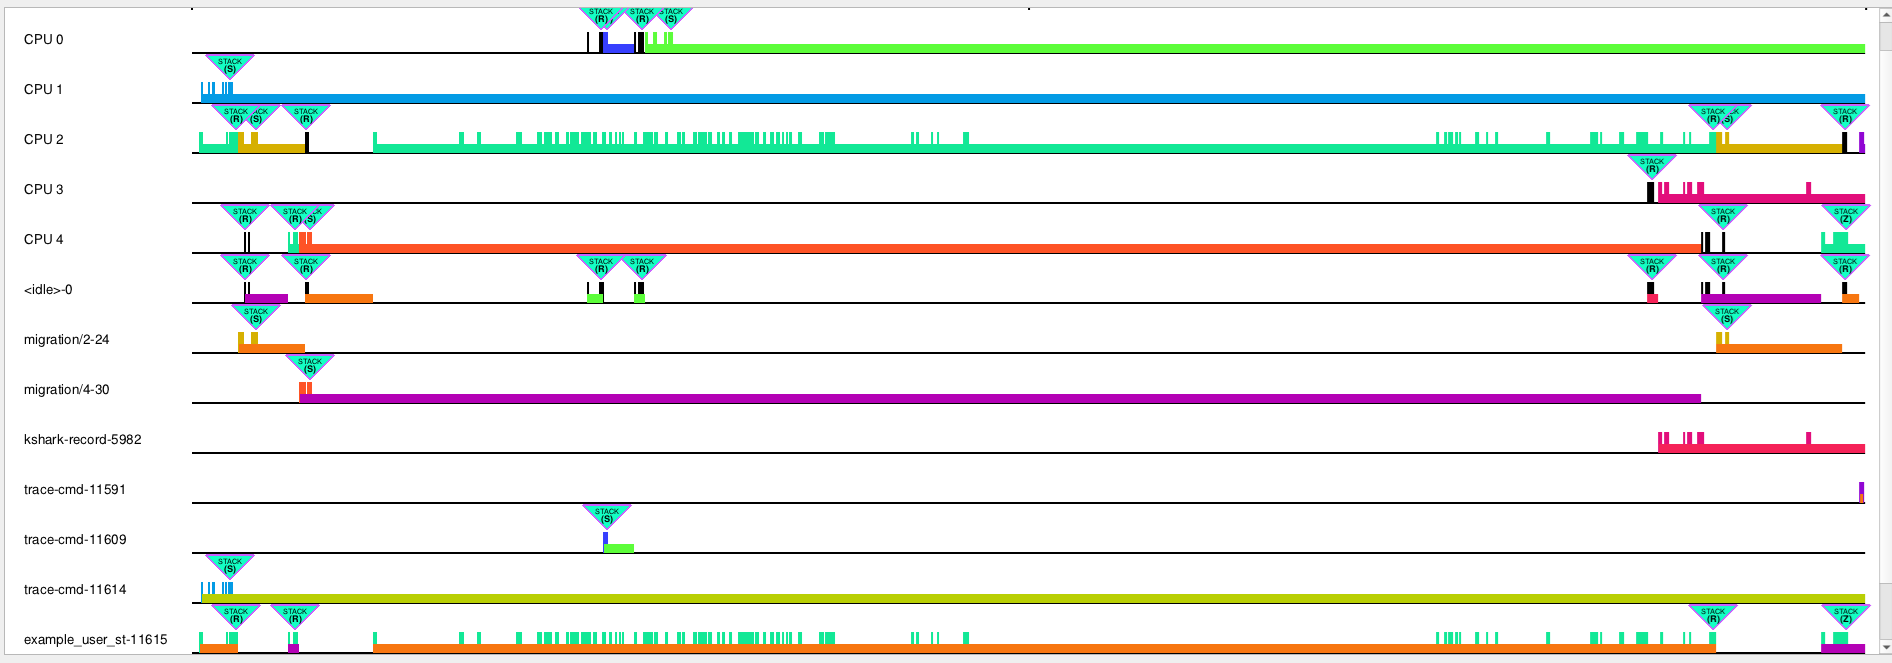
\includegraphics[width=140mm]{img/Stacklook/SlCustomDefaultColors}
      \caption{Tlačítka s konfigurovanými barvami}
      \label{SlCustomDefaultColors}
  \end{figure}

  \item \emph{Nastavení pro jednotlivé události} - Každá událost má své vlastní zaškrtávací políčko, kterým lze Stacklook zapnout nebo vypnout pro daný typ záznamu, a (pokud je k dispozici) číselník s offsetem do zásobníku kernelu, který slouží k určení \uv{nejzajímavější} oblasti v zásobníku pro danou událost. Maximální hodnota offsetu je 100~000~000 (sto milionů), minimální 0. I zde je nepravděpodobné, že by bylo třeba využít maximální hodnotu. Ve výchozím stavu jsou všechny události povoleny (zaškrtnuty) a offset je nastaven na 3.

  \begin{itemize}
    \item Připomenutí - číselník offsetu se nezobrazí, pokud je použit nemodifikovaný KernelShark.
  \end{itemize}
\end{itemize}

Tlačítko \texttt{Apply} uloží provedené změny a zavře konfigurační okno - pokud toto tlačítko nebude stisknuto, změny se neprojeví. V ovládacích prvcích konfiguračního okna se zobrazují pouze aktuálně platné hodnoty konfigurace, konfigurační okno si po zavření neaplikované změny nepamatuje. Tlačítko \texttt{Close} i tlačítko s křížkem v pravém horním rohu okna změny zahodí a okno zavřou.

U Stacklooku nelze konfigurovat:
\begin{itemize}
\item Podporované události - plugin momentálně podporuje pouze události sched/sched\_switch a sched/sched\_waking.
\item Text v oknech detailních pohledů.
\item Text tlačítek.
\item Velikost tlačítek.
\item Pozice tlačítek.
\end{itemize}

Konfigurace není persistentní. Její momentální stav se nikam neukládá, ani do relací.

\subsubsection{V grafu}

Po načtení (a případné konfiguraci) pluginu přibližme zobrazení tak, aby bylo v grafu viditelných méně záznamů, než je nastavený limit. Nad každým podporovaným záznamem se objeví tlačítko - buď ve výchozí barvě z konfigurace, nebo, pokud používáme upravený KernelShark a máme zapnutou příslušnou část nastavení, bude tlačítko obarveno podle procesu. Používání barev procesů je plně kompatibilní s barevným posuvníkem KernelSharku.

Plugin nezobrazí tlačítka nad nepodporovanými událostmi nebo pokud podporovaná událost nenajde záznam zásobníku, ze kterého by bylo možné čerpat data.

\emph{Pokud používáme modifikovaný KernelShark}, přejeďme kurzorem nad libovolné tlačítko a informační řádek KernelSharku. Obsah řádku se změní a zobrazí:
\begin{itemize}
  \item Název procesu jako první (nejlevější) položku.
  \item Položku v zásobníku kernelu na pozici danou konfigurovaným offsetem od vrcholu zásobníku.
  \item Položku v zásobníku kernelu následující po první.
  \item Položku v zásobníku kernelu následující po druhé.
  \item A nakonec buď tři tečky \texttt{...}, pokud stack obsahuje další položky, nebo zprávu \texttt{(End of stack)}, pokud už žádné další položky nezbývají.
\end{itemize}

Pohleďme na obrázek~\ref{SlMouseHover} s malou ukázkou této funkcionality. Součástí je také okno Stacklooku (o nich více níže) a záznam zásobníku kernelu v hlavním okně v seznamu všech událostí. Vše je takto uspořádáné, aby bylo zřejmé, že položky v informačním řádku skutečně pocházejí ze zásobníku (použitý offset byl výchozí, tedy 3). Červený kruh zvýrazňuje záznam, nad kterým právě kurzor myši přejíždí.

\begin{figure}[p]\centering
    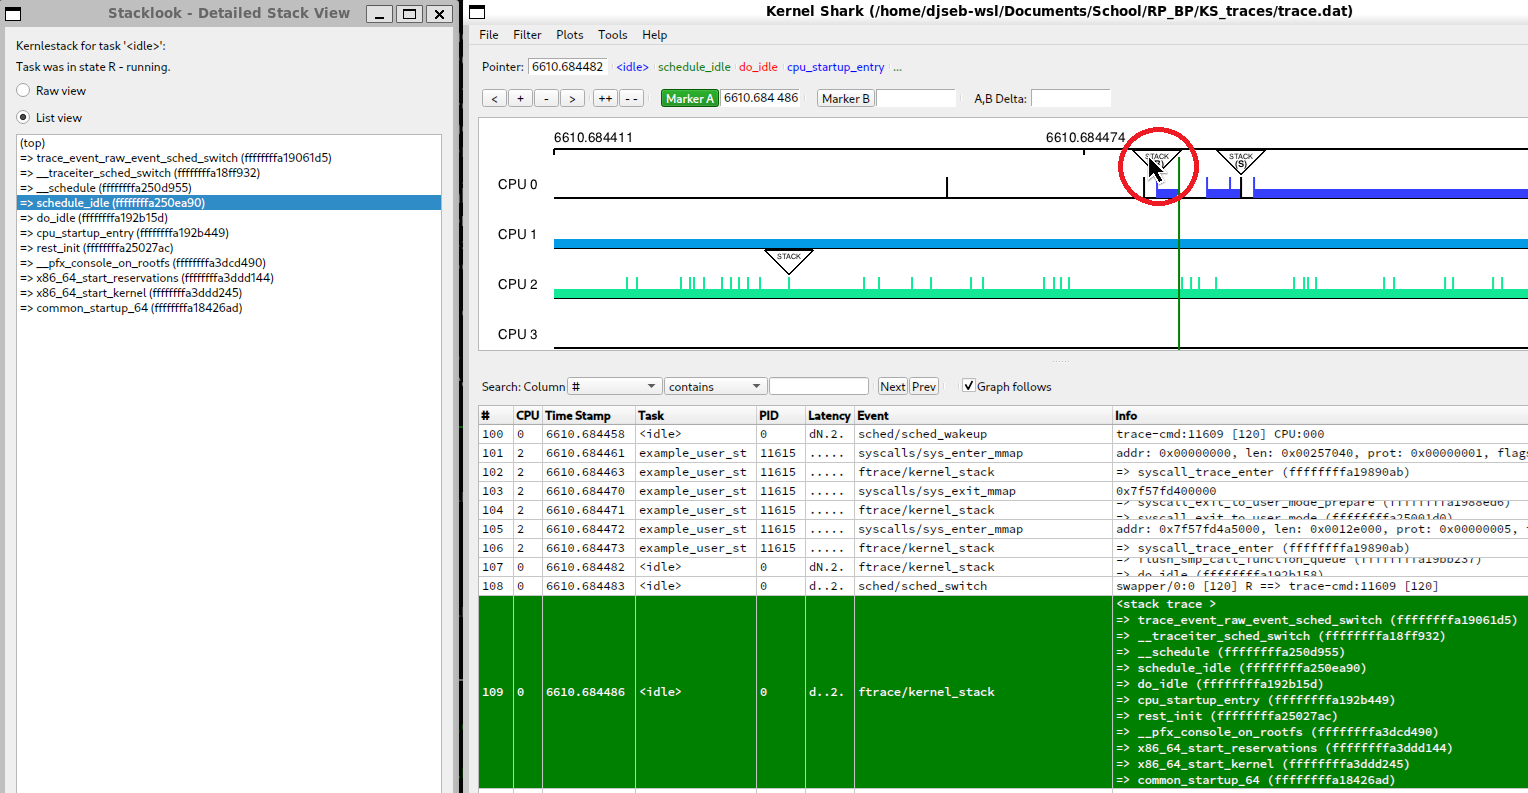
\includegraphics[width=140mm]{img/Stacklook/SlMouseHover}
    \caption{Reakce tlačítek na přejetí kurzorem myši}
    \label{SlMouseHover}
\end{figure}

Offset lze nastavit i tak vysoko, že se v náhledu zobrazí pouze poslední jedna, dvě nebo tři položky, případně žádná. V takovém případě Stacklook zobrazí pouze mínus a zprávu \texttt{(End of stack)} (viz obrázek~\ref{SlTooBigOffset}).

\begin{figure}[p]\centering
    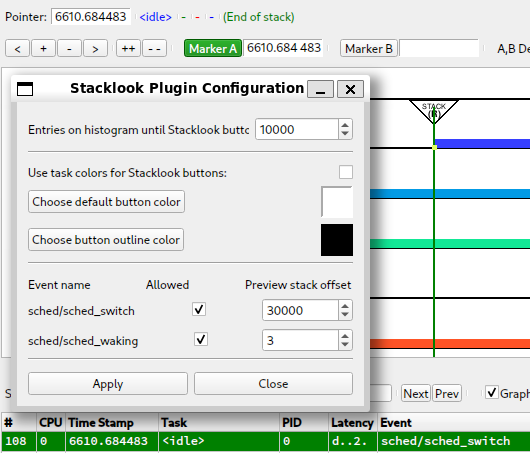
\includegraphics[width=140mm]{img/Stacklook/SlTooBigOffset}
    \caption{Chování informačního řádku při velkém offsetu do zásobníku}
    \label{SlTooBigOffset}
\end{figure}

Po dvojkliku na tlačítko Stacklooku se otevře nové okno detailního pohledu, také nazývané okno Stacklooku. Poku čteme odshora, tak v okně nejprve vidíme, že si prohlížíme zásobník kernelu nějakého procesu. Níže je napsáno, zda byl proces probuzen (zobrazuje se pouze u událostí sched/sched\_waking) nebo o jejím předchozím stavu (pouze u událostí sched/sched\_switch). Následují dvě rádiová tlačítka a zobrazení zásobníku kernelu k dané události. Rádiová tlačítka přepínají mezi různými způsoby zobrazení zásobníku:
\begin{itemize}
  \item Ve výchozím stavu je zobrazení ve formě surového textu, tedy zásobník je pouze řetězec s konci řádků. Toto je užitečné pro zkopírování zásobníku jako jednoho textu nebo pro zvýraznění konkrétní části položky v zásobníku.
  \item Alternativně lze zásobník zobrazit jako seznam, což umožňuje jednodušší a rychlejší (namísto dvojitého kliknutí stačí jedno) zvýraznění jednotlivých položek.
\end{itemize}

Pro jeden záznam může být otevřeno více oken, zároveň může být otevřeno více oken pro různé záznamy, v libovolné kombinaci.

Vše popsáno výše si můžeme prohlédnout na obrázku~\ref{SlMultipleWindowsMultipleViewsTwoSameEntires}.

\begin{figure}[p]\centering
    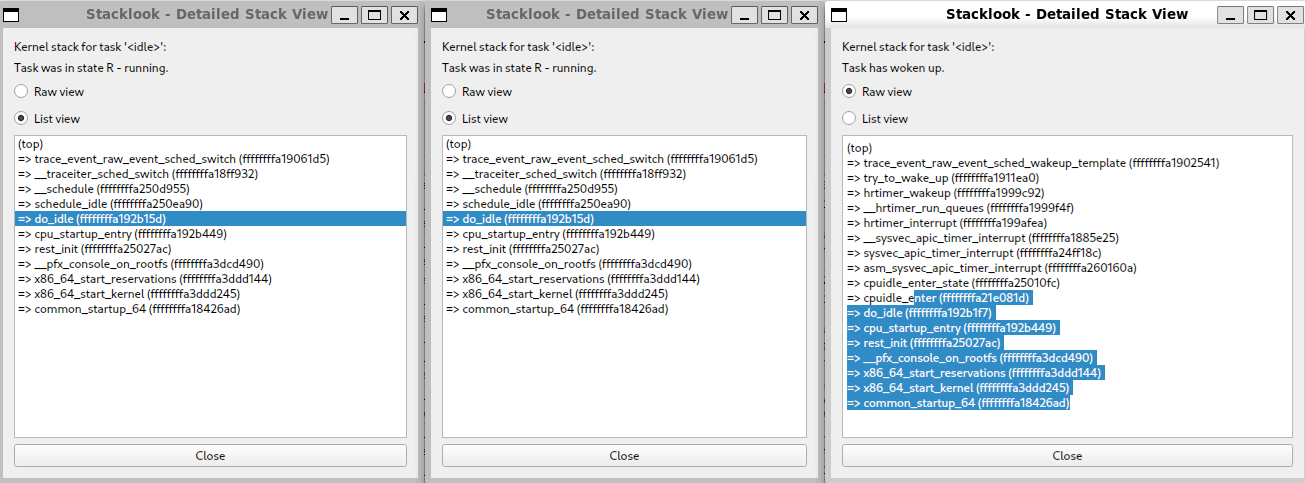
\includegraphics[width=140mm]{img/Stacklook/SlMultipleWindowsMultipleViewsTwoSameEntires}
    \caption{Několik oken detailních pohledů představující svou strukturu}
    \label{SlMultipleWindowsMultipleViewsTwoSameEntires}
\end{figure}

Okno lze zavřít přes tlačítko \texttt{Close} v dolní části okna, nebo pomocí tlačítka s křížkem v hlavičce okna. Všechna okna se zavřou, pokud bude zavřeno hlavní okno KernelSharku.

Pro přehled předchozích stavů, které jsou napsány v detailních pohledech pro sched\_switch události, je níže jejich seznam s krátkým vysvětlením každého z nich.
\begin{itemize}
  \item Uninterruptible (disk) sleep - úroces čeká na dostupnost zdrojů a nereaguje na signály.
  \item Idle - pro speciální vlákno kernelu, nelze převést do stavu Running.
  \item Parked - pouze pro procesy kernelu, proces se dobrovolně vzdá CPU a označí se tímto stavem, aby mohl být spuštěn později. 
  \item Running - proces běží na nějakém CPU.
  \item Sleeping - proces čeká na dostupnost zdrojů a reaguje na signály.
  \item Stopped - procesu byl zaslán STOP signál.
  \item Tracing stop - proces se zastavil, jelikož je právě trasován či laděn.
  \item Dead - přechodný stav těsně předtím, než bude proces dealokován.
  \item Zombie - proces skončil svou práci a čeká na uklizení rodičovským procesem.
\end{itemize}

\subsection{Doporučení}

\begin{itemize}
  \item Vždy načtěme Stacklook před načtením relace. Může to programu ušetřit nepříjemná překvapení.
  \item Neotvírejme stovky a stovky oken Stacklooku, pokud nechceme zbytečně zatížit paměť.
  \item Nedoporučuje se nastavovat příliš vysoký limit záznamů v histogramu v konfiguraci. Jinak by plugin mohl používat příliš mnoho paměti kvůli velkému množství naráz dostupných tlačítek Stacklooku.
  \item I když relace v KernelSharku fungují, jsou trochu nestabilní. Tento plugin se snaží jejich vnitřní logiku nenarušovat, ale varuje, že pokud plugin není načten předem, mohou nastat neočekávané problémy. Například načtení relace s aktivním pluginem nepřidá do menu \texttt{Tools} odpovídající položku pro vyvolání konfiguračního okna.
\end{itemize}

\section{Bugy a chyby}

Pokud by se tlačítka Stacklook překrývala, bude tlačítko příslušící \emph{starší} události vykresleno nad tlačítkem pro událost \emph{pozdější}, avšak kliknutí nebo najetí myší na překryté tlačítko použije k interakci tlačítko pro \emph{pozdější} událost. Podle autorových znalostí jde o interní chování KernelSharku, které nelze na straně pluginu opravit.

Načtení relace KernelSharku, kde byl Stacklook aktivní, bez předchozího načtení pluginu způsobí \emph{segmentation fault} a \emph{pád programu} při najetí kurzoru myši na Stacklook tlačítka.

\section{Rozšíření}
Tato sekce se podívá na některá další vylepšení, která by pluginu prospěla nebo jej zjednodušila.

\subsubsection*{Více událostí}
Plugin lze rozšířit o další podporované události. Hlavními místy pro tato rozšíření je pak propojující modul, kde se podporované události sbírají a do kontextu se ukládají jejich identifikátory, a mapová konstanta s hodnotami informací specifických pro typ události, která je uvnitř funkci tlačítek, jež vytváří detailní pohledy.

\subsubsection*{Persistentní konfigurace}
Konfigurace pluginu není persistentní, což je nepříjemné, pokud jsme u konfigurace pluginu měnili mnoho věcí. Pokud si je chceme zachovat, musíme nechat program běžet, což bude hlavně u velkých trasovacích dat zbytečně namáhat hardware. Jistě by pomohlo, kdyby bylo možné konfiguraci pluginu ukládat do relací KernelSharku, nebo do nějakých vlastních konfiguračních souborů.

\section{Kritika}
V této sekci jsou sepsány kritiky, které napadly autora pluginu. K nim jsou buď připsány obrany a nebo přiznání, že kritika má své místo a nejspíše bylo lepší vydat se jiným směrem. Upozorňujeme, že kritika může očekávat, že její čtenář viděl implementaci řešení popsaného v této práci.

\subsubsection*{Konfigurační singleton}
Použití singletonu v tomto případě dává smysl, konfigurace musí být vždy jen jedna a hodí se, když je globálně dostupná. Návrhový vzor není ovšem bez chyb. Hlavními neduhy pak jsou obtížná testovatelnost a skryté závislosti v implementaci. Návrh konfigurace se alespoň snaží zajistit, že konfigurační objekt nemůže být změněn jinak, než skrze GUI. Tím zakážeme alespoň skryté změny konfigurace a lze se spolehnout na jediný zdroj změn, zmíněnou GUI. To také znamená, že neexistuje jiný způsob změny konfigurace, třeba skrze kód. Není tak možné vytvořit nějaký jiný plugin, který by měnil konfiguraci Stacklooku. To není špatně a plugin počítá s tím, že na něm nebudou ostatní pluginy záviset.

\subsubsection*{Verze pluginu pro nemodifikovaný KernelShark}
Je možné se dívat na tuto část pluginu jako zbytečnou práci navíc, která v kódu pluginu vytváří zmatky kvůli použití maker pro podmíněnou kompilaci. Cílem této verze byla přístupnost pluginu širší veřejnosti. Plugin, ačkoliv ne kompletní, plní své hlavní funkce i pokud pár drobností není k dispozici, jako například barvení tlačítek dle barev procesů. Jistě existují uživatelé, kteří jsou ochotni vyzkoušet plugin, ale nikoliv pozměněný KernelShark, třeba už jen ze strachu bezpečnosti provedených změn. Plugin se svou verzí pro nemodifikovaný KernelShark je právě pro tyto uživatele. Tak plugin může pomoci více uživatelům - což je hlavním cílem všech vylepšení.

\subsubsection*{Špatný záznam zásobníku pro událost}
Stacklook se při prvním kreslení pokusí najít záznamy zásobníků. Pokud se mu toto podaří, dá odkaz na záznam události záznamu zásobníku záznamu události, která záznamu zásobníku předchází. Problémem je, že pokud se pro nějakou událost záznam zásobníku ztratí, nebo se posune k jinému záznamu zásobníku, pak je možné, že dvě události potom budou sdílet stejný záznam události záznamu zásobníku, přičemž jedné z nich nebude doopravdy patřit. Taková situace při testování pluginu nenastala, ale není ani nemožná (jak Trace-cmd, tak KernelShark dokážou alespoň detekovat, které události byly ztraceny, tzn. že by se mohla ztratit i událost záznamu zásobníku). 

\section{Zhodnocení splnění požadavků}
Plugin zřejmě splňuje obecné cíle pluginů, tj. vlastní adresář s instrukcemi k sestavení a nezávislost na jiných pluginech (nikde v analýze jsme se nerozhodli použít nějaký z dalších pluginů jako závislost a ani jsme nepřišli na konflikty s jinými pluginy). V analýze jsme pak postupovali tak, abychom každý z cílů splnili. Navíc jsme nepřišli na žádné problémy při vytváření řešení. Tím jsme splnili i požadavky vlastní.